\documentclass[tikz]{standalone}

\usepackage{fontspec}

\usetikzlibrary{arrows}
\usetikzlibrary{calc}
\usetikzlibrary{decorations.pathreplacing}
\usetikzlibrary{positioning}
\usetikzlibrary{matrix}

\usepackage{fontspec}

\begin{document}

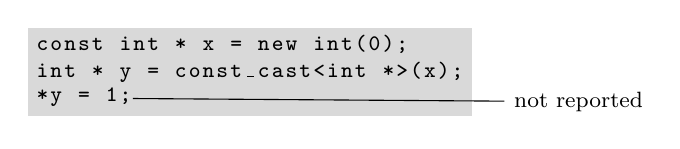
\begin{tikzpicture}
  [node distance=5mm, >=stealth',
  every node/.style={font=\footnotesize},
  every matrix/.style={fill=black!15, inner sep=1mm, row sep=0.5mm,
                        matrix of nodes, nodes in empty cells,
                        minimum height=0.5em, minimum width=.5em,
                        nodes={anchor=base, inner sep=0, font=\ttfamily\footnotesize}}]

  \matrix (snippet) {
c & o & n & s & t &   & i & n & t &   & * &   & x &   & = &   & n & e & w &   & i & n & t & ( & 0 & ) & ; &   &   &   &   \\
i & n & t &   & * &   & y &   & = &   & c & o & n & s & t & \_ & c & a & s & t & < & i & n & t &   & * & > & ( & x & ) & ; \\
* & y &   & = &   & 1 & ; &   &   &   &   &   &   &   &   &   &   &   &   &   &   &   &   &   &   &   &   &   &   &   &   \\
  };

  \node (comment)  [right=of snippet-3-31] {not reported};

  \path (snippet-3-7) edge (comment);
\end{tikzpicture}

\end{document}
